% Provenance (never printed): see sources/outline_sources.md (Year 2: energy geology --- the
% petroleum system quantified, unconventional resources, geothermal systems, uranium deposits,
% geological storage of carbon dioxide).
% Kerogen kinetics and elemental analyses: Fletcher and Pugmire (DOE, OSTI 1176871); kerogen
% types and Easy%Ro: Advanced Chemistry Basins Project (DOE, OSTI 830009); maturity thresholds:
% USGS MF-2008-B; TTI: Waples (1980) and Hammerschmidt et al. (2014); volumetrics and CO2
% storage: DOE/NETL (2008) and IPCC SRCCS (2005) chapter 5; geothermal: USGS OFR 2008-1296 and
% FS 2008-3082; uranium: USGS Bulletin 1693; Oklo: OSTI abstract records. Ledger rows in
% sources/ledger/book4.md; curves from figdata/bachelor-2/maturation.py and co2_density.py,
% numbers from the Book 4 second-writer scratch calculator calc/ch30.py.
% Geology and sourced numbers only: no advocacy, no policy.
\chapter{Geologia da energia}\label{ch:b2:energy-geology}

O petróleo é o resto de organismos microscópicos, soterrados com lama e cozidos durante milhões de anos a
cerca de \qty{100}{\celsius}; a energia geotérmica é esse mesmo calor da Terra, captado diretamente.
Ambos são regidos pela temperatura e pelo tempo: o primeiro pela velocidade de uma reação química à medida que
as rochas soterradas se aquecem lentamente, o segundo pela quantidade de calor que um volume de rocha armazena e pela rapidez com que a água
consegue levá-lo a um poço. Este capítulo quantifica o sistema petrolífero, passa aos recursos aos quais
falta um de seus elementos, ao calor geotérmico e ao urânio, e termina com a operação inversa:
devolver o dióxido de carbono ao subsolo.
% ledger: earle:oil-window, earle:organic-preservation

\begin{recall}
\textbf{Dos volumes escolares}: rocha geradora, querogênio, maturação, janela do petróleo, migração,
rocha reservatório, rocha selante, armadilha, sobrecarga, sistema petrolífero; o carvão e seu grau de carbonificação; a energia geotérmica.
\textbf{Do volume do primeiro ano}: o fluxo de calor e o geotermo; a porosidade e a permeabilidade; a pressão
de fluido nos poros, a tensão efetiva e o critério de Coulomb; a perfilagem de poço; a bacia sedimentar e a
subsidência. \textbf{Dos livros de química}: a lei de Arrhenius, a energia de ativação, a reação de primeira
ordem. \textbf{Dos livros de física}: o decaimento radioativo, a constante de decaimento, a meia-vida; o
ponto crítico de um fluido. \textbf{Do \cref{ch:b2:basins-compared}}: a \omterm{def:b2:basins-compared:curve}{curva de subsidência}.
\textbf{Do \cref{ch:b2:ore-deposits}}: o \omterm{def:b2:ore-deposits:types}{tipo de jazida}, a \omterm{def:b2:ore-deposits:grade}{tonelagem}.
\end{recall}

\section{O sistema petrolífero quantificado}\label{sec:b2:energy-geology:petroleum}

Um sistema petrolífero precisa de uma rocha geradora rica em querogênio, de um reservatório, de uma rocha selante, de uma armadilha e de
sobrecarga suficiente para aquecer a rocha geradora, e seus eventos devem ocorrer na ordem certa: a armadilha deve
existir quando o petróleo migra. Quantificá-lo significa responder a três perguntas: que \omterm{def:b2:energy-geology:kerogen}{tipo de querogênio}
a rocha geradora contém, até que ponto ele foi convertido, e quanto do produto está na
armadilha.
% ledger: magoon00:tps

\begin{definition}[Tipo de querogênio, diagrama de van Krevelen]\label{def:b2:energy-geology:kerogen}
Os querogênios dividem-se em três \emph{tipos de querogênio}\index{tipo de querogênio} segundo sua composição elementar:
o tipo~I, sapropélico, o mais rico em hidrogênio, que gera sobretudo óleo; o tipo~III, húmico ou carbonoso,
pobre em hidrogênio, que gera sobretudo metano; e o tipo~II, intermediário, fonte de óleo
e de gás. O \emph{diagrama de van Krevelen}\index{diagrama de van Krevelen} representa a razão atômica H/C de
um querogênio em função de sua razão atômica O/C; os tipos ocupam regiões diferentes dele, e a maturação
desloca um querogênio para H/C baixa e O/C baixa.
\end{definition}

Sete querogênios imaturos de tipo conhecido, analisados num mesmo estudo de laboratório, têm H/C atômica de
1.51 e 1.61 (tipo~I, entre eles o folhelho betuminoso de Green River, em Utah, depositado em lagos e rico em
restos de algas), 1.22 a 1.28 (tipo~II, entre eles a Kimmeridge Clay do mar do Norte),
1.13 (um tipo misto II/III) e 0.99 (tipo~III, o carvão de Cameo, no Colorado). O querogênio de Green
River, com \qty{77}{\percent} de carbono em massa, tem em média a fórmula C$_{100}$H$_{150}$N$_3$O$_8$S: H/C 1.50 e
O/C 0.08. Aquecido em laboratório a \qty{10}{K} por minuto, deixa um resíduo cuja H/C cai para
1.20 a \qty{460}{\celsius} e para 0.54 a \qty{525}{\celsius}, enquanto sua O/C cai de 0.08 para cerca de
0.01: o caminho traçado à esquerda da figura abaixo.
% ledger: acb04:kerogens, fp14:gr-kerogen, fp14:gr-chars, mf88:thresholds
% values: GR3.9 kerogen H/C 1.486, O/C 0.080; chars 460 C 1.200/0.016, 525 C 0.544/0.011 (figdata maturation.py vk)

\begin{omfigure}
\centering
\begin{minipage}[b]{0.49\linewidth}\centering
\begin{tikzpicture}
\begin{axis}[omrecord, width=0.95\linewidth, height=5.0cm, xmin=0, xmax=0.12, ymin=0, ymax=1.8,
  xlabel={O/C atômica}, ylabel={H/C atômica}, xtick={0,0.04,0.08}, scaled x ticks=false,
  xticklabel style={/pgf/number format/fixed}, tick label style={font=\scriptsize},
  label style={font=\small}]
% computed in figdata/bachelor-2/maturation.py part vk; ledger: fp14:gr-kerogen, fp14:gr-chars
\addplot[omThm, line width=0.9pt, mark=*, mark size=1.3pt, -{Stealth[length=4pt]}] table[x=oc, y=hc] {figdata/out/bachelor-2-maturation-vk.dat};
\node[font=\scriptsize, text=omThm, anchor=north east] at (axis cs:0.081,1.45) {querogênio};
\node[font=\scriptsize, text=omThm, anchor=west] at (axis cs:0.013,0.52) {\qty{525}{\celsius}};
% ledger: acb04:kerogens (H/C of immature kerogens; O/C not reported)
\draw[omThm, line width=1pt] (axis cs:0.104,1.51) -- (axis cs:0.12,1.51);
\draw[omThm, line width=1pt] (axis cs:0.104,1.61) -- (axis cs:0.12,1.61);
\draw[omProp, line width=1pt] (axis cs:0.104,1.22) -- (axis cs:0.12,1.22);
\draw[omProp, line width=1pt] (axis cs:0.104,1.25) -- (axis cs:0.12,1.25);
\draw[omProp, line width=1pt] (axis cs:0.104,1.28) -- (axis cs:0.12,1.28);
\draw[omExo, line width=1pt] (axis cs:0.104,1.13) -- (axis cs:0.12,1.13);
\draw[omDef, line width=1pt] (axis cs:0.104,0.99) -- (axis cs:0.12,0.99);
\node[font=\scriptsize, text=omThm, anchor=east] at (axis cs:0.103,1.58) {I};
\node[font=\scriptsize, text=omProp, anchor=east] at (axis cs:0.103,1.25) {II};
\node[font=\scriptsize, text=omDef, anchor=east] at (axis cs:0.103,0.97) {III};
\end{axis}
\end{tikzpicture}
\end{minipage}\hfill
\begin{minipage}[b]{0.49\linewidth}\centering
\begin{tikzpicture}
\begin{axis}[omrecord, width=0.95\linewidth, height=5.0cm, xmin=60, xmax=220, ymin=0, ymax=1,
  xlabel={temperatura (\unit{\celsius})}, ylabel={taxa de transformação},
  tick label style={font=\scriptsize}, label style={font=\small}]
% computed in figdata/bachelor-2/maturation.py part tr; ledger: fp14:gr-daem
\addplot[black!40, densely dotted] coordinates {(60,0.5) (220,0.5)};
\addplot[omDef, line width=1.1pt] table[x=t_c, y=tr1] {figdata/out/bachelor-2-maturation-tr.dat};
\addplot[omThm, line width=1.1pt] table[x=t_c, y=tr10] {figdata/out/bachelor-2-maturation-tr.dat};
\addplot[omDef, line width=0.6pt, densely dashed] table[x=t_c, y=app1] {figdata/out/bachelor-2-maturation-tr.dat};
\addplot[omThm, line width=0.6pt, densely dashed] table[x=t_c, y=app10] {figdata/out/bachelor-2-maturation-tr.dat};
\node[font=\scriptsize, text=omDef, anchor=east] at (axis cs:125,0.80) {\qty{1}{\celsius\per\Myr}};
\node[font=\scriptsize, text=omThm, anchor=west] at (axis cs:160,0.30) {\qty{10}{\celsius\per\Myr}};
\end{axis}
\end{tikzpicture}
\end{minipage}
\par\smallskip{\small À esquerda: um \omterm{def:b2:energy-geology:kerogen}{diagrama de van Krevelen}. O caminho vermelho é o do querogênio de tipo~I de Green River
e de seus resíduos após aquecimento em laboratório a \qty{10}{K} por minuto até 400--\qty{525}{\celsius};
os traços à direita marcam a H/C de sete querogênios imaturos de tipo~I (vermelho), II (laranja),
II/III (cinza) e III (azul), cuja O/C não foi informada. Dados: Fletcher e Pugmire (2014);
Advanced Chemistry Basins Project (2004). À direita: taxa de transformação do querogênio de Green River
aquecido a taxas constantes a partir de \qty{10}{\celsius}, com sua distribuição de energias de ativação
(contínua) e só com sua energia média, segundo \eqref{eq:b2:energy-geology:maturation} (tracejada).}
\end{omfigure}

A conversão do querogênio em petróleo é um conjunto de reações de primeira ordem, cada uma obedecendo à
lei de Arrhenius. Numa bacia em subsidência a temperatura de uma rocha geradora sobe de modo lento e quase
constante, o que faz do resultado a seguir o núcleo dos modelos de maturação.

\begin{proposition}[Reação de primeira ordem a taxa de aquecimento constante]\label{prop:b2:energy-geology:maturation}
Seja uma reação de primeira ordem de constante de velocidade $k = A\,e^{-E/RT}$ num material aquecido à
taxa constante $\beta = \mathrm{d}T/\mathrm{d}t$ a partir de uma temperatura $T_0$ na qual $k$ é desprezível.
A fração não convertida à temperatura $T$ é
\begin{equation}
x(T) = \exp\Bigl[-\frac{A}{\beta}\int_{T_0}^{T} e^{-E/RT'}\,\mathrm{d}T'\Bigr]
\approx \exp\Bigl[-\frac{A R T^2}{\beta E}\,e^{-E/RT}\Bigr] ,
\label{eq:b2:energy-geology:maturation}
\end{equation}
valendo a aproximação quando $E/RT \gg 1$; a taxa de transformação é $1 - x$.
\end{proposition}

\begin{proof}
Ser de primeira ordem significa que $\mathrm{d}x/\mathrm{d}t = -k x$. Com $\mathrm{d}t = \mathrm{d}T/\beta$,
$\mathrm{d}\ln x = -(A/\beta)\,e^{-E/RT}\,\mathrm{d}T$, e integrar a partir de $x = 1$ em $T_0$ dá
a primeira forma. Quanto à integral, $\frac{\mathrm{d}}{\mathrm{d}T}\bigl[\frac{RT^2}{E}e^{-E/RT}\bigr]
= \bigl(1 + \frac{2RT}{E}\bigr)e^{-E/RT}$, de modo que a integral vale $\frac{RT^2}{E}e^{-E/RT}$ a menos de uma
correção relativa da ordem de $2RT/E$, sem contribuição do limite inferior, pois $e^{-E/RT_0} \ll
e^{-E/RT}$.
\end{proof}

Seguem-se duas consequências. A conversão ocorre numa faixa estreita de temperatura, porque
$e^{-E/RT}$ varia muito depressa (exercício~\ref{exo:b2:energy-geology:11}). E um aquecimento mais lento converte
a uma temperatura mais baixa: fazendo $x = 1/2$, uma taxa de aquecimento dez vezes maior eleva a temperatura de
meia conversão em cerca de $(RT^2/E)\ln 10$. A cinética do querogênio de Green River, ajustada à
pirólise de laboratório, é $A = \qty{9.21e13}{s^{-1}}$ e $E/R = \qty{26800}{K}$ ($E =
\qty{223}{kJ/mol}$); com essa energia única, a meia conversão ocorre a \qty{136.4}{\celsius} para
\qty{1}{\celsius\per\Myr} e a \qty{150.9}{\celsius} para \qty{10}{\celsius\per\Myr}, um deslocamento de
\qty{14.5}{\celsius} contra $6.26 \times \ln 10 = \qty{14.4}{K}$ previstos. Aquecido a
\qty{10}{K} por minuto, o mesmo querogênio converte-se perto de \qty{450}{\celsius}
(exercício~\ref{exo:b2:energy-geology:6}): o tempo substitui a temperatura, e é por isso que a cinética é
medida por pirólise a cerca de 250 a \qty{600}{\celsius}, e que extrapolá-la ao longo de doze
ordens de grandeza em taxa de aquecimento deixa incerta a profundidade prevista da janela do petróleo.
% ledger: fp14:gr-daem, acb04:kinetic-spread, codata:R
% values: Thalf 136.403 / 150.873 C; RT2/E 6.2587 K; lab 445.9 C (figdata maturation.py numbers, calc/ch30.py)

Um querogênio real contém ligações de muitas energias, de modo que sua cinética é uma distribuição de energias
de ativação, cada fração obedecendo à proposição; para o querogênio de Green River a distribuição é
normal, com desvio-padrão $\sigma/R = \qty{481}{K}$. A distribuição alarga a
conversão, como mostra a direita da figura: a \qty{150}{\celsius} o querogênio aquecido a
\qty{1}{\celsius\per\Myr} está \qty{93}{\percent} convertido, o aquecido dez vezes mais depressa
\qty{48}{\percent}.
% ledger: fp14:gr-daem
% values: TR 0.927 / 0.484 at 150 C (figdata maturation.py numbers)

\begin{definition}[Refletância da vitrinita, índice tempo--temperatura]\label{def:b2:energy-geology:maturity}
A \emph{refletância da vitrinita}\index{refletância da vitrinita}, $R_o$, é a porcentagem da luz
incidente refletida por grãos polidos de vitrinita, um componente orgânico do carvão e do querogênio,
medida ao microscópio; ela cresce irreversivelmente com o aquecimento e registra a maior maturidade térmica que uma rocha atingiu. O
\emph{índice tempo--temperatura}\index{índice tempo--temperatura} (TTI) de Lopatin é a soma
$\sum_n \Delta t_n\,2^n$ sobre os intervalos de \qty{10}{\celsius} que uma rocha atravessou,
sendo $\Delta t_n$ o tempo em milhões de anos passado no intervalo de número $n$, com $n = 0$
para 100 a \qty{110}{\celsius}, $n = 1$ para 110 a \qty{120}{\celsius}, $n = -1$ para 90 a
\qty{100}{\celsius}, e assim por diante.
\end{definition}

Na escala de refletância, a geração de óleo pelos querogênios de tipos~I e II começa perto de $R_o =
\qty{0.60}{\percent}$; acima de 1.20 a \qty{1.30}{\percent} o óleo é instável e decompõe-se em
metano; o tipo~III começa a produzir metano perto de \qty{0.73}{\percent}, e a geração de gás prossegue até
cerca de \qty{4.8}{\percent}. Os modelos calculam $R_o$ como um querogênio: o modelo Easy\%Ro
trata a vitrinita como vinte reações paralelas de primeira ordem com $A = \qty{e13}{s^{-1}}$ e energias
de 34 a \qty{72}{kcal/mol} (142 a \qty{301}{kJ/mol}), e converte sua fração convertida $F$,
no máximo 0.85, em $R_o = \exp(-1.6 + 3.7F)$, que vai de 0.20 a \qty{4.7}{\percent}.
% ledger: mf88:thresholds, acb04:easyro, fp14:gr-chars

A refletância é calculada da mesma maneira ao longo de cada horizonte de uma bacia. Na bacia inventada da
figura abaixo, os sedimentos acumularam-se a \qty{100}{m} por milhão de anos de 100 a \qty{70}{\Ma},
depois a \qty{35}{m} por milhão de anos, sob uma superfície a \qty{10}{\celsius} e com um gradiente constante
de \qty{30}{\celsius\per\km}. Seu horizonte mais antigo atingiu $R_o = \qty{0.6}{\percent}$ a
\qty{67.6}{\Ma}, a \qty{3080}{m} e \qty{102}{\celsius}, e \qty{1.3}{\percent} a
\qty{11.6}{\Ma}, a \qty{5040}{m} e \qty{161}{\celsius}; hoje ele está a \qty{5450}{m} e
\qty{173.5}{\celsius}, com $R_o = \qty{1.54}{\percent}$. Como o geotermo é estacionário, as
frentes de refletância seguem quase as isotermas, e o início da geração de óleo fica perto de
\qty{100}{\celsius}, dentro dos 60 a \qty{120}{\celsius} dos volumes escolares.
% ledger: acb04:easyro, mf88:thresholds, earle:settings, earle:oil-window
% values: figdata maturation.py numbers (oldest_ro06_*, oldest_ro13_*, ro_oldest_now)

\begin{omfigure}
\centering
\begin{tikzpicture}
\begin{axis}[omrecord, width=0.86\linewidth, height=4.8cm, xmin=0, xmax=100, ymin=0, ymax=5.6,
  x dir=reverse, y dir=reverse, ylabel={profundidade (km)}, xticklabels={}, name=bh,
  tick label style={font=\scriptsize}, label style={font=\small}]
% computed in figdata/bachelor-2/maturation.py parts burial and fronts (invented basin)
\addplot[black!40, densely dashed] coordinates {(100,1.333) (0,1.333)};
\addplot[black!40, densely dashed] coordinates {(100,3.0) (0,3.0)};
\addplot[black!40, densely dashed] coordinates {(100,4.667) (0,4.667)};
\node[font=\tiny, text=black!60, anchor=south east, fill=white, inner sep=1pt] at (axis cs:1,1.333) {\qty{50}{\celsius}};
\node[font=\tiny, text=black!60, anchor=south east, fill=white, inner sep=1pt] at (axis cs:1,3.0) {\qty{100}{\celsius}};
\node[font=\tiny, text=black!60, anchor=south east, fill=white, inner sep=1pt] at (axis cs:1,4.667) {\qty{150}{\celsius}};
\addplot[black!70, line width=0.5pt, unbounded coords=jump] table[x=t_ma, y expr=\thisrow{d90}/1000] {figdata/out/bachelor-2-maturation-burial.dat};
\addplot[black!70, line width=0.5pt, unbounded coords=jump] table[x=t_ma, y expr=\thisrow{d80}/1000] {figdata/out/bachelor-2-maturation-burial.dat};
\addplot[black!70, line width=0.5pt, unbounded coords=jump] table[x=t_ma, y expr=\thisrow{d70}/1000] {figdata/out/bachelor-2-maturation-burial.dat};
\addplot[black!70, line width=0.5pt, unbounded coords=jump] table[x=t_ma, y expr=\thisrow{d60}/1000] {figdata/out/bachelor-2-maturation-burial.dat};
\addplot[black!70, line width=0.5pt, unbounded coords=jump] table[x=t_ma, y expr=\thisrow{d50}/1000] {figdata/out/bachelor-2-maturation-burial.dat};
\addplot[black!70, line width=0.5pt, unbounded coords=jump] table[x=t_ma, y expr=\thisrow{d40}/1000] {figdata/out/bachelor-2-maturation-burial.dat};
\addplot[black!70, line width=0.5pt, unbounded coords=jump] table[x=t_ma, y expr=\thisrow{d30}/1000] {figdata/out/bachelor-2-maturation-burial.dat};
\addplot[black!70, line width=0.5pt, unbounded coords=jump] table[x=t_ma, y expr=\thisrow{d20}/1000] {figdata/out/bachelor-2-maturation-burial.dat};
\addplot[black!70, line width=0.5pt, unbounded coords=jump] table[x=t_ma, y expr=\thisrow{d10}/1000] {figdata/out/bachelor-2-maturation-burial.dat};
\addplot[black, line width=1.1pt, unbounded coords=jump] table[x=t_ma, y expr=\thisrow{d100}/1000] {figdata/out/bachelor-2-maturation-burial.dat};
\addplot[omDef, line width=1.4pt, unbounded coords=jump] table[x=t_ma, y expr=\thisrow{z06}/1000] {figdata/out/bachelor-2-maturation-fronts.dat};
\addplot[omThm, line width=1.4pt, unbounded coords=jump] table[x=t_ma, y expr=\thisrow{z13}/1000] {figdata/out/bachelor-2-maturation-fronts.dat};
\node[font=\scriptsize, text=omDef, anchor=north, fill=white, inner sep=1pt] at (axis cs:40,3.05) {$R_o = \qty{0.6}{\percent}$};
\node[font=\scriptsize, text=omThm, anchor=north west, fill=white, inner sep=1pt] at (axis cs:9,5.10) {\qty{1.3}{\percent}};
\node[font=\scriptsize, anchor=north east, fill=white, inner sep=1pt] at (axis cs:58,4.75) {rocha geradora};
\end{axis}
\begin{axis}[at={(bh.south west)}, anchor=north west, yshift=-0.15cm, width=0.86\linewidth,
  height=2.9cm, xmin=0, xmax=100, ymin=0.4, ymax=6.6, x dir=reverse, y dir=reverse,
  xlabel={tempo (\unit{\Ma})}, ytick={1,2,3,4,5,6},
  yticklabels={rocha geradora, rocha reservatório, rocha selante, sobrecarga, formação da armadilha, geração},
  tick label style={font=\tiny}, label style={font=\small}, axis line style={black!60},
  xtick={100,80,60,40,20,0}]
% schematic events chart of the same invented basin
\fill[omLithShale!80!black] (axis cs:100,0.75) rectangle (axis cs:96,1.25);
\fill[omLithSand!70!black] (axis cs:90,1.75) rectangle (axis cs:85,2.25);
\fill[omLithShale!80!black] (axis cs:85,2.75) rectangle (axis cs:80,3.25);
\fill[black!25] (axis cs:80,3.75) rectangle (axis cs:0,4.25);
\fill[omProp!70] (axis cs:75,4.75) rectangle (axis cs:70,5.25);
\fill[omDef!70] (axis cs:67.6,5.75) rectangle (axis cs:11.6,6.25);
\end{axis}
\end{tikzpicture}
\par\smallskip{\small Em cima: história de soterramento de uma bacia inventada (em preto: horizontes depositados a cada
10 milhões de anos, o mais espesso sendo a rocha geradora), isotermas (tracejadas), e as profundidades onde
o Easy\%Ro atinge \qty{0.6}{\percent} (azul) e \qty{1.3}{\percent} (vermelho). Embaixo: seu quadro de
eventos; a geração vai de $R_o = \qty{0.6}{\percent}$ a \qty{1.3}{\percent} na rocha geradora,
depois da formação da armadilha.}
\end{omfigure}

O TTI é mais antigo e mais grosseiro. Ele supõe que a maturação dobra de velocidade a cada
\qty{10}{\celsius}, como faz uma lei de Arrhenius com $E \approx \qty{82}{kJ/mol}$ perto de
\qty{100}{\celsius} (exercício~\ref{exo:b2:energy-geology:5}); em sua escala, Waples situou o início
da geração de óleo num TTI de 15, seu pico em 75 e seu fim em 160.
% ledger: waples80:tti, hamm14:tti-table

\begin{method}[Calcular um índice tempo--temperatura]\label{met:b2:energy-geology:tti}
Os dados são a história de soterramento da rocha geradora e o geotermo, suposto estacionário.
\begin{enumerate}
  \item \textbf{Caminho de temperatura.} Converta a profundidade em temperatura a cada instante: temperatura da superfície
        mais gradiente vezes profundidade.
  \item \textbf{Tempos nos intervalos.} Encontre o tempo $\Delta t_n$ passado em cada intervalo de
        \qty{10}{\celsius}; onde a taxa de aquecimento $\beta$ é constante, $\Delta t_n = \qty{10}{\celsius}/\beta$.
  \item \textbf{Soma.} Some os produtos $\Delta t_n\,2^n$ em ordem cronológica; o início, o pico e o
        fim da geração de óleo são atingidos quando a soma acumulada passa de 15, 75 e 160.
\end{enumerate}
\end{method}

Os modelos de bacia exprimem a conversão como uma taxa de transformação: a fração do potencial
de hidrocarbonetos original de uma rocha geradora já convertida. Num modelo de uma bacia californiana,
supôs-se que a expulsão da rocha geradora começava a uma taxa de \qty{10}{\percent}, atingia o pico a
\qty{50}{\percent} e terminava a \qty{95}{\percent}. O óleo expulso, mais leve que a água,
migra para cima até rochas reservatório permeáveis, e fica retido onde uma rocha selante fecha uma armadilha.
% ledger: peters08b4:tr, magoon00:tps, earle:migration-traps

\begin{proposition}[Óleo in situ]\label{prop:b2:energy-geology:volumetrics}
Sejam uma armadilha de área $A$ e um reservatório de espessura útil $h$, porosidade $\phi$ e saturação em água
$S_w$, e seja $B_o$ o fator volume-formação de seu óleo, a razão entre o volume que uma quantidade
de óleo ocupa no reservatório e seu volume na superfície. O \emph{volume de óleo inicialmente in situ
em condições de tanque}\index{volume de óleo inicialmente in situ em condições de tanque}, o volume de óleo medido na superfície, é
\begin{equation}
\mathrm{STOIIP} = \frac{A\,h\,\phi\,(1 - S_w)}{B_o} .
\label{eq:b2:energy-geology:stoiip}
\end{equation}
\end{proposition}

\begin{proof}
O volume total do reservatório é $Ah$ e seu volume poroso $Ah\phi$; uma fração $1 - S_w$ dos
poros contém óleo, de modo que o óleo ocupa $Ah\phi(1 - S_w)$ no reservatório, e $1/B_o$ vezes isso
na superfície.
\end{proof}

\begin{definition}[Fator de recuperação]\label{def:b2:energy-geology:volumetrics}
O \emph{fator de recuperação}\index{fator de recuperação} de um reservatório é a fração do óleo (ou do gás)
inicialmente in situ que é produzida ao longo de sua vida.
\end{definition}

A produção primária e a recuperação secundária por injeção de água recuperam juntas, tipicamente, de 30 a \qty{40}{\percent} do óleo in situ; a injeção de dióxido
de carbono recupera de 10 a \qty{15}{\percent} a mais. Uma armadilha de \qty{10}{km^2} com \qty{30}{m} de espessura útil
de reservatório, porosidade 0.20, saturação em óleo 0.70 e $B_o = 1.2$ contém \qty{3.5e7}{m^3} de óleo
em condições de tanque, dos quais de 1.05 a \qty{1.4e7}{m^3} seriam produzidos.
% ledger: netl08:oilgas

\section{Recursos não convencionais}\label{sec:b2:energy-geology:unconventional}

\begin{definition}[Reservatório não convencional]\label{def:b2:energy-geology:unconventional}
Um \emph{reservatório não convencional}\index{reservatório não convencional} é uma rocha de permeabilidade tão
baixa que o óleo ou o gás contido em seus poros microscópicos não consegue fluir até um poço a uma vazão
econômica sem estimulação artificial; ele é produzido por poços perfurados horizontalmente ao longo dele e
fraturados hidraulicamente. O óleo e o gás de folhelho estão contidos na própria rocha geradora, o gás \textit{tight} em
arenitos e carbonatos de baixa permeabilidade.
\end{definition}

Uma acumulação não convencional é portanto uma rocha geradora, ou uma rocha ao lado dela, que reteve parte do que
gerou. O produto que ela contém decorre de sua maturidade: um folhelho na janela do petróleo contém óleo,
um que passou de $R_o \approx \qty{1.3}{\percent}$, gás. A produção de gás de folhelho em grande escala começou por volta de
2000 no Barnett Shale, no Texas, e a maior parte do crescimento da produção de gás dos Estados Unidos desde
2005 veio da perfuração horizontal e do fraturamento hidráulico em folhelhos, arenitos, carbonatos e
outras formações de baixa permeabilidade; também se produz gás de camadas de carvão.
% ledger: eia:shale-gas, eia:gas-coalbed, mf88:thresholds

\section{A energia geotérmica}\label{sec:b2:energy-geology:geothermal}

\begin{definition}[Sistema geotérmico, calor in situ, classes de entalpia, EGS]\label{def:b2:energy-geology:geothermal}
Um \emph{sistema geotérmico}\index{sistema geotérmico} é um volume da crosta onde calor,
permeabilidade e água se reúnem de modo que água quente ou vapor possam ser produzidos por poços. O
\emph{calor in situ}\index{calor in situ} de um reservatório é o calor que ele cederia ao se resfriar
de sua temperatura até uma temperatura de referência. Um \emph{recurso de alta entalpia}\index{recurso de alta entalpia}
é um sistema geotérmico acima de cerca de \qty{150}{\celsius}; um \emph{recurso de baixa
entalpia}\index{recurso de baixa entalpia}, um sistema abaixo de cerca de \qty{90}{\celsius}; entre os dois o
recurso é chamado de média entalpia. As três classes servem ao uso direto do calor, mas em geral só as classes média
e alta podem gerar eletricidade. Um \emph{sistema geotérmico estimulado}\index{sistema geotérmico estimulado} (EGS) é um corpo de
rocha quente de baixa permeabilidade natural no qual a permeabilidade é criada por engenharia, de modo que a água
possa circular através dele e seu calor seja recuperado.
\end{definition}
% ledger: usgs08g:classes, usgs08g:egs

\begin{proposition}[Calor in situ e potência recuperável]\label{prop:b2:energy-geology:heat}
Um reservatório de volume $V$, temperatura média $T_R$ e capacidade térmica volumétrica $C$ (rocha e fluido
dos poros juntos) contém, acima da temperatura de referência $T_0$, o calor
\begin{equation}
q_R = C\,V\,(T_R - T_0) .
\label{eq:b2:energy-geology:heat}
\end{equation}
Se uma fração $R_g$ dele chega às cabeças de poço ao longo de um tempo de produção $\tau$, a potência
térmica média produzida é $P = R_g\,q_R/\tau$.
\end{proposition}

\begin{proof}
Um volume $\mathrm{d}V$ à temperatura $T$ libera $C\,\mathrm{d}V\,(T - T_0)$ ao se resfriar até $T_0$;
somando sobre o reservatório com $C$ uniforme obtém-se $C\,V\,(T_R - T_0)$, sendo $T_R$ a temperatura
média. A potência é o calor recuperado dividido pelo tempo.
\end{proof}

As avaliações de recursos usam esse método volumétrico com uma referência de \qty{15}{\celsius}. O \omterm{def:b2:energy-geology:volumetrics}{fator de
recuperação} $R_g$ é a parte incerta: as primeiras avaliações adotavam 0.25, entre 0 e 0.5; a produção de
reservatórios fraturados aponta para cerca de 0.1, entre 0.05 e 0.2. Com $C = \qty{2.5}{MJ.m^{-3}.K^{-1}}$
(as matrizes rochosas contêm de 2 a \qty{3}{MJ.m^{-3}.K^{-1}}), um reservatório de $3 \times 4 \times
\qty{1}{km}$ a \qty{220}{\celsius} contém \qty{6.15e18}{J}; com $R_g = 0.1$ ao longo de 30 anos ele
fornece uma potência térmica média de \qty{650}{MW}. Os campos convencionais geram de 10 a
\qty{20}{MW} de eletricidade por quilômetro quadrado de campo.
% ledger: usgs08g:volume, delaney86b4:properties, usgs08g:egs
% values: 6.15e18 J; 6.15e17 J; 649.6 MW (calc/ch30.py)

Os \omterm{def:b2:energy-geology:geothermal}{sistemas geotérmicos} naturais precisam tanto de permeabilidade quanto de calor. A maioria dos grandes fica perto das
bordas das placas tectônicas, entre vulcões, fumarolas, fontes termais e gêiseres, e sua
permeabilidade é tipicamente a de fraturas abertas por falhas ativas: a água subterrânea aquecida em profundidade
sobe por elas, e os poços captam o reservatório fraturado, como no corte abaixo. Um EGS não precisa de reservatório natural:
seus poços, perfurados até cerca de \qty{5}{km}, atingem rocha quente cuja permeabilidade é criada por engenharia, e
uma avaliação dos Estados Unidos de 2008 estimou seu potencial provisório em \qty{517800}{MW} de
eletricidade, contra \qty{9057}{MW} dos sistemas convencionais identificados.
% ledger: eia:geo-where, usgs08g:egs, usgs08g:volume

\begin{omfigure}
\centering
\begin{minipage}[b]{0.55\linewidth}\centering
\begin{tikzpicture}[x=0.95cm, y=0.82cm, font=\scriptsize]
% schematic, not to scale
\fill[omLithSand!60] (0,0) -- (7,0) -- (7,-3.6) -- (0,-3.6) -- cycle;
\fill[omProp!35] (1.2,-1.05) .. controls (2.6,-0.85) and (4.4,-0.85) .. (5.8,-1.05)
  -- (5.8,-2.3) .. controls (4.4,-2.5) and (2.6,-2.5) .. (1.2,-2.3) -- cycle;
\fill[omThm!70] (2.6,-3.6) .. controls (2.8,-2.8) and (4.2,-2.8) .. (4.4,-3.6) -- cycle;
\draw[black, line width=0.8pt] (0,0) -- (7,0);
\foreach \x in {1.6,2.4,3.2,4.0,4.8,5.4} {\draw[black!55] (\x,-1.1) -- (\x+0.35,-2.2);}
\draw[omDef, line width=0.9pt, -{Stealth[length=4pt]}] (0.4,-0.1) .. controls (0.5,-2) and (1,-3) .. (2.4,-3.2);
\draw[omDef, line width=0.9pt, -{Stealth[length=4pt]}] (6.6,-0.1) .. controls (6.5,-2) and (6,-3) .. (4.6,-3.2);
\draw[omThm, line width=0.9pt, -{Stealth[length=4pt]}] (3.5,-2.85) -- (3.5,-1.2);
\draw[omThm, line width=0.9pt, -{Stealth[length=4pt]}] (3.5,-1.0) .. controls (3.6,-0.6) .. (5.4,0.02);
\draw[black, line width=1.1pt] (2.9,0.25) -- (2.9,-1.6);
\draw[black, line width=1.1pt] (4.3,0.25) -- (4.3,-1.7);
\fill[black] (2.75,0.25) rectangle (3.05,0.45);
\fill[black] (4.15,0.25) rectangle (4.45,0.45);
\node[anchor=south] at (5.4,0.05) {fonte termal};
\node[anchor=south] at (2.9,0.45) {poço};
\node[anchor=south] at (4.3,0.45) {poço};
\node[text=omDef, anchor=north west] at (0.05,-2.35) {recarga};
\node[text=omDef, anchor=north west] at (0.05,-2.65) {fria};
\node[align=center, fill=omProp!20, inner sep=1pt] at (5.1,-1.62) {reservatório\\fraturado};
\node[text=white] at (3.5,-3.35) {intrusão};
\end{tikzpicture}
\end{minipage}\hfill
\begin{minipage}[b]{0.40\linewidth}\centering
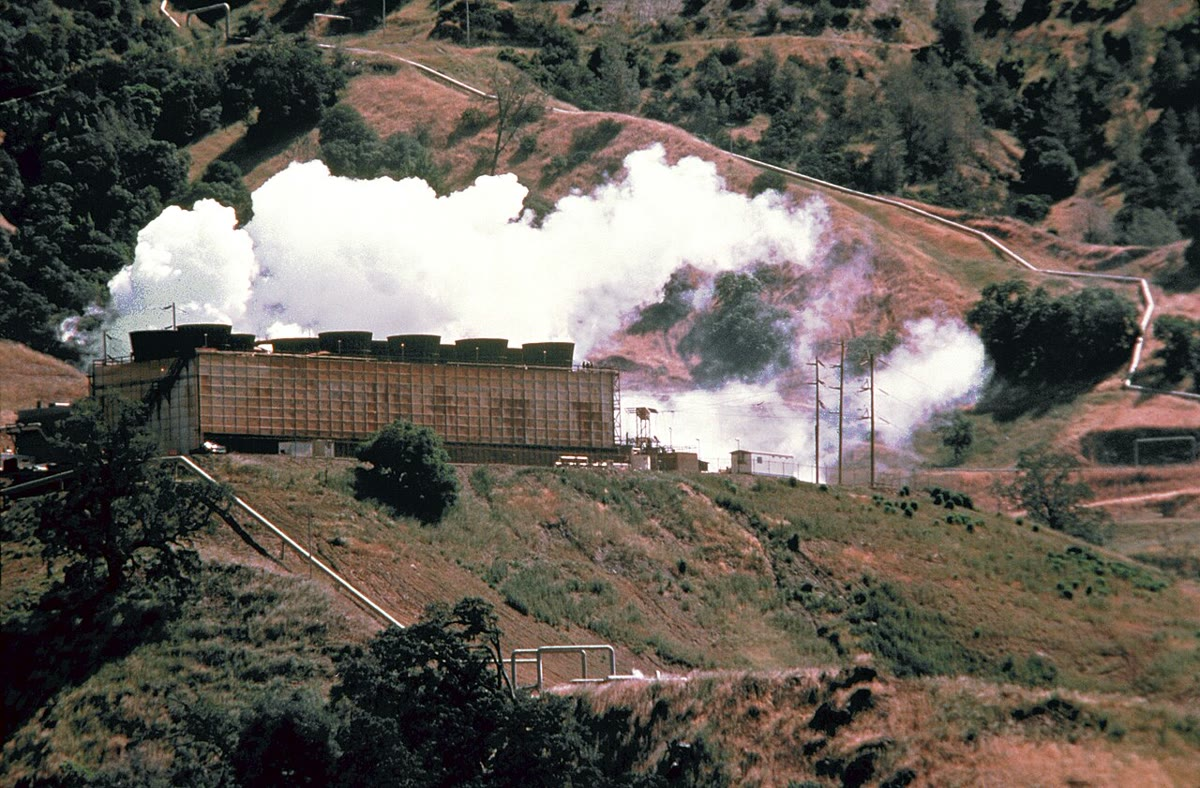
\includegraphics[width=\linewidth]{images/book4/b2-30-geyserville.jpg}
\end{minipage}
\par\smallskip{\small À esquerda: um \omterm{def:b2:energy-geology:geothermal}{sistema geotérmico} de alta entalpia (esquemático, sem escala): a água
recarregada nas margens (azul) é aquecida sobre uma intrusão e sobe por um reservatório fraturado
(vermelho) até uma fonte termal; poços captam o reservatório. À direita: uma usina geotérmica perto de Geyserville,
Califórnia, em 1982, com tubulações de vapor na encosta. Fotografia: Departamento de Defesa dos EUA
(domínio público).}
\end{omfigure}
% ledger: photo:b2-30-geyserville, usgs08g:egs

\begin{definition}[Sismicidade induzida]\label{def:b2:energy-geology:induced}
A \emph{sismicidade induzida}\index{sismicidade induzida} é a atividade sísmica causada por operações
humanas que mudam a tensão ou a pressão de fluido nos poros da crosta, na maioria das vezes a
injeção de fluido no subsolo.
\end{definition}

O mecanismo é o critério de Coulomb com pressão de fluido nos poros: uma falha desliza quando a tensão cisalhante
atinge $\mu(\sigma_n - p)$, de modo que elevar $p$ leva à ruptura uma falha já tensionada
sem nenhuma mudança da carga tectônica. Nos anos 1960, fluidos residuais injetados no embasamento
pré-cambriano fraturado sob o Rocky Mountain Arsenal, perto de Denver, a profundidades de 3.7 a
\qty{7.0}{km}, desencadearam sismos; eles ficaram confinados à parte do reservatório onde a
pressão havia subido mais de \qty{32}{bar} (\qty{3.2}{MPa}). O forte aumento dos sismos
de Oklahoma foi atribuído ao descarte de águas residuais: quatro poços de alto volume
poderiam explicar um quinto da sismicidade do centro dos Estados Unidos, desencadeando
sismos a mais de \qty{30}{km} de distância. A estimulação de um reservatório EGS eleva a pressão nos poros da
mesma maneira, de propósito.
% ledger: hb81:denver, keranen:oklahoma, usgs08g:egs

\section{O urânio}\label{sec:b2:energy-geology:uranium}

Dois \omterm{def:b2:ore-deposits:types}{tipos de jazida} ilustram como o urânio se concentra: um numa discordância antiga, o
outro em arenito.

\begin{definition}[Jazidas de urânio associadas a discordância e de tipo roll-front]\label{def:b2:energy-geology:uranium}
Uma \emph{jazida de urânio associada a discordância}\index{jazida de urânio associada a discordância} é um corpo
de pechblenda e uraninita que preenche fraturas e brechas em pelitos carbonosos metamorfizados e
nos quartzo-arenitos sobrejacentes, abaixo, acima ou através de uma discordância entre rochas do \omterm{def:b2:precambrian-earth:eons}{Proterozoico}
Inferior e Médio numa \omterm{def:b2:basins-compared:types}{bacia intracratônica}. Uma \emph{jazida de urânio de tipo roll-front}\index{jazida de urânio de tipo roll-front}
é um corpo em forma de crescente de minerais de urânio que corta o acamamento de um
arenito feldspático ou tufáceo no limite entre terreno oxidado e terreno reduzido, onde o
urânio foi depositado num ambiente localmente redutor, em meio à pirita.
\end{definition}

As \omterm{def:b2:ore-deposits:deposit}{jazidas} de discordância estão hospedadas em rochas de 1800 a \qty{1200}{\Ma}, os pelitos metamorfizados
abaixo da discordância e os arenitos não metamorfizados acima dela; suas rochas encaixantes são cloritizadas, e os xistos grafitosos que
acompanham muitas delas são fortes condutores elétricos, um alvo para os levantamentos eletromagnéticos. Key
Lake, Cluff Lake e Rabbit Lake, em Saskatchewan, e Jabiluka e Ranger, no norte da Austrália, são
exemplos. As frentes de oxirredução (roll fronts) são mais jovens, na maioria terciárias: em arenitos alimentados por cinza vulcânica félsica ou por
granito, os minerais de ferro oxidados ficam a montante do mergulho em relação à frente e os reduzidos a jusante, como nas bacias
de Wyoming e da Costa do Golfo do Texas.
% ledger: b1693:unconformity, b1693:sandstone

\begin{proposition}[O urânio-235 no passado]\label{prop:b2:energy-geology:u235}
Sejam $r_0$ a razão atômica atual $^{235}$U/$^{238}$U e $\lambda_5$, $\lambda_8$ as constantes de
decaimento dos dois isótopos. Há um tempo $t$, a razão era
\begin{equation}
r(t) = r_0\,e^{(\lambda_5 - \lambda_8)\,t} ,
\label{eq:b2:energy-geology:u235}
\end{equation}
e o $^{235}$U constituía uma fração $r/(1 + r)$ dos átomos de urânio, desprezando o traço de
$^{234}$U.
\end{proposition}

\begin{proof}
Cada um dos isótopos decai de modo exponencial: $N_5(\text{hoje}) = N_5(t)\,e^{-\lambda_5 t}$ e $N_8(\text{hoje})
= N_8(t)\,e^{-\lambda_8 t}$. Dividindo, $r_0 = r(t)\,e^{-(\lambda_5 - \lambda_8)t}$.
\end{proof}

Com $\lambda_5 = \qty{9.8485e-10}{yr^{-1}}$, $\lambda_8 = \qty{1.55125e-10}{yr^{-1}}$ e as
abundâncias atuais \qty{0.7204}{\percent} e \qty{99.2742}{\percent}, $r_0 = 0.0072567$; há \qty{2.0}{\Ga},
$r = 0.0381$ e o urânio natural continha \qty{3.67}{\percent} de $^{235}$U, cinco vezes a
proporção atual.
% ledger: amherst:constants, iaea:isotopes
% values: r 0.038144, 3.6743 % (calc/ch30.py)

\begin{history}[Um reator de dois bilhões de anos]
Em 1972, cientistas franceses que mediam minério de urânio encontraram déficits pequenos mas significativos de
$^{235}$U, que atribuíram à mina de Oklo, no Gabão. Ali, bolsões de rocha continham até
\qty{65}{\percent} de urânio com apenas metade da proporção normal de $^{235}$U, e neodímio
empobrecido em seu isótopo primordial $^{142}$Nd mas enriquecido nos isótopos 143 a 150 que a fissão
produz: reações em cadeia haviam ocorrido no minério há cerca de dois bilhões de anos, a cerca de \qty{300}{bar}
e 400 a \qty{500}{\celsius}. Conhecem-se dezesseis desses reatores naturais em Oklo e na vizinha
Bangombé, as duas únicas \omterm{def:b2:ore-deposits:deposit}{jazidas} do mundo onde foram encontrados; a matéria orgânica havia ajudado a
concentrar o urânio, e o óxido de urânio reteve no lugar a maior parte dos actinídeos e dos
produtos de fissão não voláteis desde então.
\end{history}
% ledger: oklo:curtis, oklo:cowan, oklo:gl96, oklo:nagy

\section{O armazenamento geológico do dióxido de carbono}\label{sec:b2:energy-geology:ccs}

\begin{definition}[Armazenamento geológico de \ce{CO2}, mecanismos de aprisionamento, fator de eficiência de armazenamento]\label{def:b2:energy-geology:ccs}
O \emph{armazenamento geológico de \ce{CO2}}\index{armazenamento geológico de CO$_2$} é a injeção de dióxido
de carbono em formações rochosas porosas profundas, reservatórios de óleo e gás depletados, formações salinas
profundas ou camadas de carvão, para retenção por longos períodos. Os \emph{mecanismos de aprisionamento
de \ce{CO2}}\index{mecanismos de aprisionamento de CO$_2$} que o retêm são o aprisionamento estrutural (e estratigráfico)
sob uma rocha selante; o aprisionamento residual, como fase imóvel retida nos poros por forças
capilares; o aprisionamento por solubilidade, por dissolução na água de formação; o aprisionamento mineral, por reação
com minerais formando carbonatos; e, no carvão e no folhelho, a adsorção na matéria orgânica. O \emph{fator de eficiência de armazenamento}\index{fator de eficiência de armazenamento}
$E$ de uma formação é a fração de seu volume poroso que se espera que o
\ce{CO2} injetado preencha.
\end{definition}
% ledger: srccs:retention, netl08:saline

O dióxido de carbono é um gás na superfície, mas seu ponto crítico fica a \qty{31.0}{\celsius} e
\qty{7.38}{MPa}. Ao longo de um geotermo de \qty{25}{\celsius\per\km} a partir de \qty{15}{\celsius} sob
pressão hidrostática, a temperatura passa o valor crítico a \qty{641}{m} e a pressão a
\qty{742}{m}; a densidade do \ce{CO2} puro salta de \qty{234}{kg.m^{-3}} a \qty{700}{m} para
\qty{583}{kg.m^{-3}} a \qty{900}{m}, e depois se estabiliza perto de 670 a \qty{700}{kg.m^{-3}} abaixo de
\qty{1.5}{km}. Uma tonelada ocupa \qty{534}{m^3} na superfície e \qty{1.6}{m^3} a \qty{1000}{m},
330 vezes menos; é por isso que as avaliações de armazenamento só consideram formações mais profundas que
\qty{800}{m}.
% ledger: nist:co2-critical, data:b4-co2-density, srccs:density, netl08:saline
% values: z_tc 641.2 m, z_pc 742.2 m; volume ratio 331.9 (figdata co2_density.py numbers)

\begin{omfigure}
\centering
\begin{minipage}[b]{0.49\linewidth}\centering
\begin{tikzpicture}
\begin{axis}[omrecord, width=0.95\linewidth, height=5.2cm, xmin=0, xmax=750, ymin=0, ymax=3,
  y dir=reverse, xlabel={densidade do \ce{CO2} (\unit{kg.m^{-3}})}, ylabel={profundidade (km)},
  tick label style={font=\scriptsize}, label style={font=\small}]
% computed in figdata/bachelor-2/co2_density.py part profile; ledger: data:b4-co2-density
\addplot[black!45, densely dashed] coordinates {(0,0.742) (750,0.742)};
\node[font=\tiny, text=black!60, anchor=south east] at (axis cs:745,0.73) {pressão crítica};
\addplot[omDef, line width=1.1pt, mark=*, mark size=0.9pt] table[x=rho, y expr=\thisrow{depth_m}/1000] {figdata/out/bachelor-2-co2_density-profile.dat};
\end{axis}
\end{tikzpicture}
\end{minipage}\hfill
\begin{minipage}[b]{0.49\linewidth}\centering
\begin{tikzpicture}
\begin{axis}[width=0.95\linewidth, height=5.2cm, xmin=0, xmax=4, ymin=0, ymax=100,
  axis x line=bottom, axis y line=left, axis line style={-}, axis on top,
  xlabel={tempo após a injeção (anos)}, ylabel={parte do \ce{CO2} armazenado},
  xtick={0,1,2,3,4}, xticklabels={1,10,100,1000,$10^4$}, ytick=\empty,
  tick label style={font=\scriptsize}, label style={font=\small}]
% schematic, after IPCC SRCCS (2005) Figure 5.9; ledger: srccs:trapping
% bands from the bottom: mineral, solubility, residual, structural (cumulative tops 0/0/1/5/15,
% 2/8/21/40/60, 10/30/56/80/90, 100)
\fill[omLithLime!60!black] (axis cs:0,0) -- (axis cs:1,0) -- (axis cs:2,1) -- (axis cs:3,5) -- (axis cs:4,15) -- (axis cs:4,0) -- cycle;
\fill[omDef!40] (axis cs:0,0) -- (axis cs:1,0) -- (axis cs:2,1) -- (axis cs:3,5) -- (axis cs:4,15) -- (axis cs:4,60) -- (axis cs:3,40) -- (axis cs:2,21) -- (axis cs:1,8) -- (axis cs:0,2) -- cycle;
\fill[omProp!40] (axis cs:0,2) -- (axis cs:1,8) -- (axis cs:2,21) -- (axis cs:3,40) -- (axis cs:4,60) -- (axis cs:4,90) -- (axis cs:3,80) -- (axis cs:2,56) -- (axis cs:1,30) -- (axis cs:0,10) -- cycle;
\fill[black!15] (axis cs:0,10) -- (axis cs:1,30) -- (axis cs:2,56) -- (axis cs:3,80) -- (axis cs:4,90) -- (axis cs:4,100) -- (axis cs:0,100) -- cycle;
\node[font=\scriptsize] at (axis cs:1.1,72) {estrutural};
\node[font=\scriptsize] at (axis cs:2.1,38) {residual};
\node[font=\scriptsize] at (axis cs:3.1,22) {solubilidade};
\node[font=\scriptsize, text=white, anchor=south east] at (axis cs:3.98,0.5) {mineral};
\end{axis}
\end{tikzpicture}
\end{minipage}
\par\smallskip{\small À esquerda: densidade do \ce{CO2} puro em função da profundidade ao longo de um geotermo de
\qty{25}{\celsius\per\km} a partir de \qty{15}{\celsius}, sob pressão hidrostática. Dados: NIST Chemistry
WebBook (equação de estado de Span--Wagner), nas condições do Relatório Especial do IPCC sobre Captura e
Armazenamento de Dióxido de Carbono (2005). À direita: como os mecanismos de aprisionamento repartem o \ce{CO2} armazenado
ao longo do tempo (esquemático, segundo o mesmo relatório): o aprisionamento pela rocha selante dá lugar às formas residual,
dissolvida e mineral, que são menos móveis.}
\end{omfigure}

\begin{proposition}[Capacidade de armazenamento de uma formação]\label{prop:b2:energy-geology:capacity}
Uma formação de área $A$, espessura $h$ e porosidade $\phi$, na qual o \ce{CO2} tem densidade $\rho$
e o \omterm{def:b2:energy-geology:ccs}{fator de eficiência de armazenamento} é $E$, pode armazenar a massa
\begin{equation}
M = A\,h\,\phi\,\rho\,E .
\label{eq:b2:energy-geology:capacity}
\end{equation}
Para um campo de petróleo depletado que produziu um volume em condições de tanque $N_p$, substituir o óleo produzido
volume por volume dá $M = \rho\,N_p\,B_o$.
\end{proposition}

\begin{proof}
O volume poroso é $Ah\phi$, do qual o \ce{CO2} preenche uma fração $E$, à densidade $\rho$. No
campo de petróleo, o óleo produzido ocupava $N_pB_o$ no reservatório, o volume que o \ce{CO2} passa a ocupar.
\end{proof}

Para as formações salinas profundas, as simulações dão $E$ entre 1 e \qty{4}{\percent} do volume poroso
numa faixa de confiança de 15 a 85 por cento, com mediana perto de \qty{2}{\percent}: a maior parte do espaço
poroso nunca é atingida, ou conserva sua água. Uma formação de \qty{1000}{km^2}, com \qty{50}{m} de espessura e
porosidade 0.20 a \qty{2000}{m} ($\rho = \qty{686}{kg.m^{-3}}$) armazena \qty{137}{Mt} com $E =
\qty{2}{\percent}$.
% ledger: netl08:saline, data:b4-co2-density
% values: 1e9*50*0.2*686*0.02 = 1.372e11 kg (calc/ch30.py)

Uma vez injetado, o \ce{CO2} sobe sob a rocha selante e se espalha. Atrás da pluma em migração, as forças capilares
retêm saturações residuais que podem chegar a 15 a \qty{25}{\percent} do espaço poroso;
a dissolução absorve de 20 a \qty{60}{kg} de \ce{CO2} por metro cúbico de água de formação, e em
formações de fluxo lento até \qty{30}{\percent} do \ce{CO2} injetado se dissolve em algumas dezenas de
anos. O aprisionamento por solubilidade domina ao longo de dezenas a centenas de anos, as formas iônicas ao longo de centenas a
milhares, o aprisionamento mineral ao longo de milhares a milhões: as reações com minerais carbonáticos levam dias,
com silicatos centenas a milhares de anos. O armazenamento torna-se mais seguro com o tempo, e em
locais bem escolhidos e bem geridos a retenção de \qty{99}{\percent} ou mais do \ce{CO2} ao longo de
1000 anos foi julgada provável.
% ledger: srccs:trapping, srccs:retention

\begin{dated}{2005}
Em Sleipner, no mar do Norte, a cerca de \qty{250}{km} da costa da Noruega, o \ce{CO2} separado do
gás natural do campo, cerca de \qty{9}{\percent} dele, é injetado desde outubro de 1996 na
formação Utsira, um arenito salino inconsolidado de 800 a \qty{1000}{m} abaixo do fundo do mar,
a cerca de \qty{1}{Mt} por ano. No início de 2005 mais de \qty{7}{Mt} haviam sido armazenadas, dos \qty{20}{Mt}
previstos para a vida do projeto. Levantamentos sísmicos repetidos imageiam a pluma, cuja área era então
de cerca de \qty{5}{km^2}, e mostram que a rocha capeadora acima dela a veda.
\end{dated}
% ledger: srccs:sleipner

\begin{inthefield}[Ler um poço enquanto ele é perfurado]
\centering
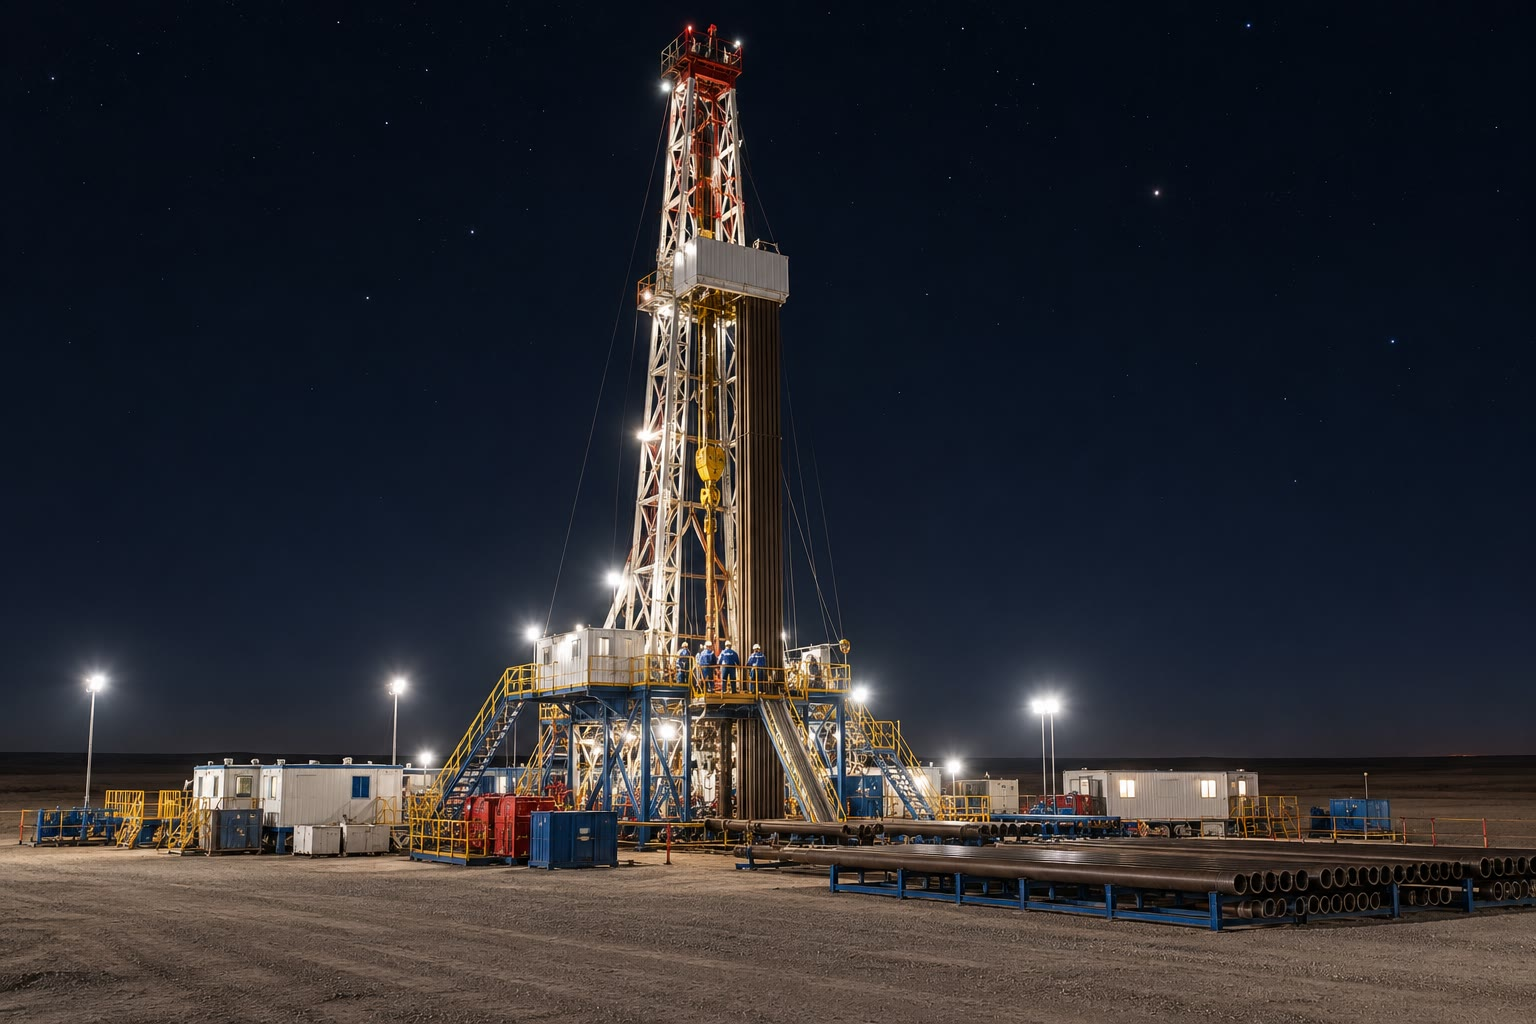
\includegraphics[width=0.56\linewidth]{images/book4/ai/b2-rig-night.jpg}
\par\smallskip{\small Uma sonda de perfuração terrestre à noite (ilustração gerada por IA).}
\par\medskip\raggedright
Quando um trecho de um poço é concluído, os geofísicos descem ferramentas num cabo e registram em função da
profundidade as propriedades das rochas em volta do furo. Uma registra sua radioatividade natural, baixa no
arenito e mais alta no folhelho; outra sua densidade total, da qual a porosidade decorre como
(densidade dos grãos $-$ densidade total)/(densidade dos grãos $-$ densidade do fluido), com \qty{2.65}{g/cm^3} para
grãos de quartzo e cerca de \qty{1}{g/cm^3} para a água. Lidos em conjunto, esses perfis de poço dão a
espessura útil do reservatório e a porosidade que entram nas fórmulas volumétricas deste capítulo.
\end{inthefield}
% ledger: keys:gamma, keys:density-porosity

\section*{Exercícios}\label{sec:b2:energy-geology:exercises}

Dados para os exercícios, salvo indicação em contrário: $R = \qty{8.314}{J.mol^{-1}.K^{-1}}$; um milhão
de anos vale \qty{3.156e13}{s}; querogênio de Green River $A = \qty{9.21e13}{s^{-1}}$, $E/R = \qty{26800}{K}$;
massas atômicas C 12.011, H 1.008, O 15.999; densidade do \ce{CO2} ao longo do perfil da figura:
\qty{1.872}{kg.m^{-3}} na superfície, 583 a \qty{900}{m}, 621 a \qty{1000}{m}, 686 a
\qty{2000}{m}. Arredonde a três algarismos significativos.
% ledger: codata:R, fp14:gr-daem, data:b4-co2-density

\begin{exercise}[$\star$]\label{exo:b2:energy-geology:1}
(a) Quatro querogênios imaturos têm H/C atômica de 1.58, 0.95, 1.24 e 1.12. Atribua um tipo a cada um e diga
qual produziria sobretudo gás. (b) Verifique as razões H/C e O/C da fórmula
C$_{100}$H$_{150}$N$_3$O$_8$S. (c) Encontre-as a partir da composição em massa C \qty{77.4}{\percent}, H
\qty{9.8}{\percent}, O \qty{8.2}{\percent}.
\end{exercise}

\begin{exercise}[$\star$]\label{exo:b2:energy-geology:2}
(a) Cinco amostras de uma rocha geradora de tipo~II têm $R_o$ = 0.45, 0.68, 1.1, 1.6 e \qty{2.5}{\percent}.
Descreva o estado de cada uma em relação ao óleo e ao gás. (b) Um querogênio de tipo~III com $R_o =
\qty{0.68}{\percent}$ está gerando metano? (c) Que fração convertida $F$ do Easy\%Ro corresponde a
$R_o = 0.6$ e a \qty{1.3}{\percent}?
\end{exercise}

\begin{exercise}[$\star$]\label{exo:b2:energy-geology:3}
Uma armadilha cobre \qty{6}{km^2}; seu reservatório tem \qty{25}{m} de espessura útil, porosidade 0.18 e saturação
em água 0.30, e $B_o = 1.25$. (a) Encontre o volume de óleo no reservatório e o STOIIP. (b) Encontre
o volume produzido para \omterm{def:b2:energy-geology:volumetrics}{fatores de recuperação} de 0.30 e 0.40.
\end{exercise}

\begin{exercise}[$\star$]\label{exo:b2:energy-geology:4}
Um aquífero arenítico de \qty{200}{m} de espessura sob \qty{10}{km^2} está a \qty{75}{\celsius}. (a) Encontre seu
\omterm{def:b2:energy-geology:geothermal}{calor in situ} acima de \qty{15}{\celsius}, com $C = \qty{2.5}{MJ.m^{-3}.K^{-1}}$. (b) A que
classe de entalpia ele pertence? (c) Encontre a potência térmica média ao longo de 30 anos para $R_g = 0.25$.
\end{exercise}

\begin{exercise}[$\star\star$]\label{exo:b2:energy-geology:5}
(a) Encontre a energia de ativação para a qual uma velocidade de Arrhenius dobra entre 100 e
\qty{110}{\celsius}. (b) Por que fator cresce a velocidade da reação de Green River no mesmo
intervalo? (c) Qual das duas regras dá mais peso ao tempo que uma rocha passou a baixa temperatura,
e o que isso implica para um TTI calculado para uma rocha geradora de tipo~I?
\end{exercise}

\begin{exercise}[$\star\star$]\label{exo:b2:energy-geology:6}
(a) Mostre a partir de \eqref{eq:b2:energy-geology:maturation} que a temperatura de meia conversão obedece a
$T = (E/R)\big/\ln\bigl[A T^2/(\beta\,(E/R)\ln 2)\bigr]$, e resolva-a por iteração para o querogênio de Green
River aquecido a \qty{1}{\celsius\per\Myr} e a \qty{10}{K} por minuto. (b) Compare a
diferença com a estimativa $(RT^2/E)\ln(\beta_2/\beta_1)$ tomada à temperatura mais baixa, e
explique a discrepância.
\end{exercise}

\begin{exercise}[$\star\star$]\label{exo:b2:energy-geology:7}
Usando \eqref{eq:b2:energy-geology:u235} e os dados do texto: (a) encontre a proporção de $^{235}$U no
urânio natural há \qty{2.0}{\Ga} e há \qty{1.8}{\Ga}; (b) quando ela era de \qty{3.00}{\percent}?
(c) O minério de Oklo contém apenas metade da proporção normal atual de $^{235}$U. Ignorando o $^{238}$U
consumido, que fração do $^{235}$U presente na época das reações sofreu fissão, e
por que o decaimento posterior não muda a resposta?
\end{exercise}

\begin{exercise}[$\star\star$]\label{exo:b2:energy-geology:8}
(a) Encontre o volume de \qty{1}{Mt} de \ce{CO2} na superfície, a \qty{1000}{m} e a
\qty{2000}{m}. (b) Em Sleipner mais de \qty{7}{Mt} haviam sido injetadas até 2005, a cerca de
\qty{900}{m}, numa pluma de área \qty{5}{km^2}. Tomando uma porosidade de 0.35 e uma saturação em \ce{CO2}
de 0.30 na pluma, encontre o volume de rocha que ela ocupa e sua espessura média.
\end{exercise}

\begin{exercise}[$\star\star$]\label{exo:b2:energy-geology:9}
Um reservatório de alta entalpia mede $3 \times 2 \times \qty{1.5}{km}$ a \qty{250}{\celsius}, com
$C = \qty{2.6}{MJ.m^{-3}.K^{-1}}$. (a) Encontre seu \omterm{def:b2:energy-geology:geothermal}{calor in situ} acima de \qty{15}{\celsius}. (b) Encontre a
potência térmica média ao longo de 30 anos para $R_g = 0.1$ e $0.25$. (c) Seu campo cobre \qty{6}{km^2};
a 10 a \qty{20}{MW} de eletricidade por quilômetro quadrado, que fração da potência térmica com
$R_g = 0.1$ se torna eletricidade?
\end{exercise}

\begin{exercise}[$\star\star\star$]\label{exo:b2:energy-geology:10}
Uma falha a cerca de \qty{4}{km} suporta uma tensão normal de \qty{80}{MPa} e uma tensão cisalhante de
\qty{22}{MPa}; seu coeficiente de atrito é 0.6 e a pressão nos poros é hidrostática,
\qty{39}{MPa}. (a) A falha é estável? Encontre o aumento de pressão nos poros que a leva à ruptura, em
megapascals e em bars, e compare com o limiar de Denver. (b) O mesmo se a tensão cisalhante for de
\qty{24}{MPa}. (c) Explique por que sismos podem ser desencadeados a quilômetros de um poço de injeção,
e anos depois do início da injeção.
\end{exercise}

\begin{exercise}[$\star\star\star$]\label{exo:b2:energy-geology:11}
(a) A partir da aproximação em \eqref{eq:b2:energy-geology:maturation}, mostre que, a uma taxa de
aquecimento constante, a taxa de transformação sobe de \qty{10}{\percent} a \qty{90}{\percent} num
intervalo de temperatura $\Delta T \approx \bigl[\ln\ln 10 - \ln\ln(10/9)\bigr]\,RT^2/E$. (b) Calcule-o
para o querogênio de Green River a \qty{1}{\celsius\per\Myr}. (c) Compare com a curva contínua da
figura e explique a diferença.
\end{exercise}

\begin{exercise}[$\star\star\star$]\label{exo:b2:energy-geology:12}
Sleipner deve armazenar \qty{20}{Mt} de \ce{CO2}. (a) Encontre o volume de água de formação necessário para
dissolvê-lo todo, a 20 e a \qty{60}{kg.m^{-3}}. (b) Encontre seu volume como fase livre a
\qty{1000}{m}. (c) Com $E = \qty{2}{\percent}$, encontre o volume poroso de formação necessário, e
a área de uma formação de \qty{50}{m} de espessura e porosidade 0.30.
\end{exercise}
% ledger: srccs:trapping, srccs:sleipner, hb81:denver

\begin{problem}[{Problema de fim de semana --- uma bacia, dois usos}]\label{pb:b2:energy-geology:1}
Numa bacia inventada, uma rocha geradora de tipo~I foi depositada a \qty{120}{\Ma} na superfície.
Os sedimentos acumularam-se depois a \qty{60}{m} por milhão de anos até \qty{70}{\Ma}, e a \qty{30}{m}
por milhão de anos desde então. A superfície está a \qty{15}{\celsius} e o geotermo é estacionário, de
\qty{25}{\celsius\per\km}. O querogênio tem a cinética de Green River do texto (energia única).
Sua cozinha de geração, a parte matura da rocha geradora, cobre \qty{400}{km^2}, tem \qty{50}{m} de espessura e
densidade \qty{2400}{kg.m^{-3}}, e pode produzir \qty{30}{kg} de óleo por tonelada de rocha com
conversão completa; o óleo tem densidade na superfície de \qty{850}{kg.m^{-3}}. O óleo preenche uma armadilha de
\qty{12}{km^2} cujo reservatório, centrado a \qty{2000}{m}, tem espessura útil de \qty{40}{m},
porosidade 0.22 e saturação em água 0.25, com $B_o = 1.30$. Use os dados dos exercícios; arredonde a
três algarismos significativos.

\noindent\textbf{Parte I --- Soterramento e índice tempo--temperatura.}
\begin{enumerate}
  \item Encontre a profundidade e a temperatura da rocha geradora a \qty{70}{\Ma} e hoje.
  \item Encontre sua taxa de aquecimento em cada fase.
  \item Encontre o tempo que ela passou em cada intervalo de \qty{10}{\celsius}, de \qty{15}{\celsius} até
        sua temperatura atual.
  \item Calcule seu TTI hoje (método do texto).
  \item Quando, a que temperatura e a que profundidade ela passou um TTI de 15?
  \item O mesmo para 75 e 160.
  \item Pelo TTI, a rocha geradora ainda está gerando óleo?
\end{enumerate}

\noindent\textbf{Parte II --- A conversão pela cinética.}
\begin{enumerate}[resume]
  \item Encontre a constante de velocidade a \qty{90}{\celsius} e mostre que menos de \qty{0.2}{\percent} do
        querogênio pode ter sido convertido antes de \qty{70}{\Ma}.
  \item Usando \eqref{eq:b2:energy-geology:maturation} com a taxa de aquecimento da segunda fase,
        encontre a fração não convertida e a taxa de transformação hoje.
  \item Encontre a temperatura de meia conversão a essa taxa de aquecimento (exercício~\ref{exo:b2:energy-geology:6}).
  \item Quando ela foi atingida?
  \item Compare com a época do pico de geração dada pelo TTI, e explique a diferença.
  \item Um querogênio de tipo~II com energia de ativação média mais baixa teria se convertido mais cedo ou mais tarde?
\end{enumerate}

\noindent\textbf{Parte III --- Óleo gerado, in situ e recuperável.}
\begin{enumerate}[resume]
  \item Tomando uma taxa de transformação de 0.92, encontre a massa de óleo gerada na cozinha de geração.
  \item Encontre seu volume na superfície.
  \item Encontre o STOIIP da armadilha.
  \item Que fração do óleo gerado a armadilha contém? Mantenha \qty{1.56e9}{m^3} para (15).
  \item Encontre o óleo produzido para um \omterm{def:b2:energy-geology:volumetrics}{fator de recuperação} de 0.35.
  \item Por que o \omterm{def:b2:energy-geology:volumetrics}{fator de recuperação} é muito menor que um, e o que mudaria a injeção de \ce{CO2}?
\end{enumerate}

\noindent\textbf{Parte IV --- O campo depletado como reservatório de \ce{CO2}.}
\begin{enumerate}[resume]
  \item Encontre a temperatura e a pressão hidrostática do reservatório. O \ce{CO2} injetado está
        supercrítico ali? Leia sua densidade na figura.
  \item Mantendo $N_p = \qty{2.13e7}{m^3}$, encontre o volume de reservatório liberado pela produção.
  \item Exprima-o como um \omterm{def:b2:energy-geology:ccs}{fator de eficiência de armazenamento} do volume poroso da armadilha, e compare com
        as formações salinas.
  \item Uma formação salina sob o campo cobre \qty{600}{km^2}, tem \qty{80}{m} de espessura,
        porosidade 0.20, com \ce{CO2} a \qty{691}{kg.m^{-3}}. Encontre sua capacidade com $E =
        \qty{2}{\percent}$.
  \item Quantos anos de injeção ao ritmo de Sleipner a preencheriam?
  \item Com $\rho = \qty{686}{kg.m^{-3}}$ e o volume liberado arredondado para \qty{2.77e7}{m^3}, encontre
        a capacidade de armazenamento de \ce{CO2} do reservatório depletado, em megatoneladas.
\end{enumerate}
\end{problem}
% ledger: fp14:gr-daem, waples80:tti, hamm14:tti-table, netl08:oilgas, netl08:saline, data:b4-co2-density, nist:co2-critical, srccs:sleipner
